\documentclass[twoside,12pt]{article}
\usepackage[left=3.3cm,top=3.7cm,right=3.3cm,bottom=3.7cm,footskip=1.1cm]{geometry}

\newcommand{\omissis}{[\ldots\negthinspace]}

\renewcommand{\baselinestretch}{1}
\usepackage[utf8]{inputenc}
\usepackage{setspace}
\usepackage{amssymb}
\usepackage{ragged2e}
\usepackage{xcolor}
\usepackage{hyperref}
  
\usepackage{geometry}
\usepackage{pifont}
\usepackage{amsmath}
\usepackage{lastpage}
\usepackage{adjustbox}
\usepackage{abstract}
\usepackage{anyfontsize}
\usepackage{breqn}
\usepackage{multirow}
\usepackage{caption}
\usepackage{graphicx}
\usepackage{subfig}
\usepackage{tabularx}
\usepackage{fancyhdr}
\usepackage{xcolor}
\usepackage{eurosym}
\usepackage{natbib}
%\bibliographystyle{agsm}
\bibliographystyle{aer}  % AER style
\usepackage{booktabs}

\makeatletter
\newenvironment{chapquote}[2][2em]
  {\setlength{\@tempdima}{#1}%
   \def\chapquote@author{#2}%
   \parshape 1 \@tempdima \dimexpr\textwidth-2\@tempdima\relax%
   \itshape}
  {\par \normalfont\hfill--\ \chapquote@author\hspace*{\@tempdima}\par\bigskip}
\makeatother

\pagestyle{fancy}
\fancyhf{}
\renewcommand{\headrulewidth}{0pt}
\fancyhead[RO,LE]{\large \thepage}
\fancyhead[CO]{\textit{\large Geographic Variation in Childhood Obesity}}
\fancyhead[CE]{\textit{\large Samuele Giambra}}
\fancyfoot[L,C,R]{}



\fancypagestyle{firststyle}
{
   \fancyhf{}
   \fancyfoot[C]{\large \thepage}
   \renewcommand{\headrulewidth}{0pt}
}
  
\newcommand{\yourname}{Samuele Giambra}
\newcommand{\youremail}{\url{giambar@hotmail.com}}

\hypersetup{urlcolor=blue!50!black}

%%%%%%%%%%%%%%%%%%%%%%%%%%%%%%%%%%%%%%%%%%
%here introduce cooler section titles  and abstract
\renewcommand{\thesection}{\Roman{section}} 
\renewcommand{\thesubsection}{\thesection.\Alph{subsection}}

\usepackage{titlesec}
\titleformat{\section}
  {\large\bfseries\centering}{\thesection.}{0.2em}{}
\titleformat{\subsection}
  {\normalfont\itshape\centering}{\thesubsection.}{0.3em}{}
 \titleformat{\subsubsection}
  {\normalfont\bfseries\itshape}{\thesubsubsection.}{0.3em}{}
  
\renewcommand{\abstractname}{}    % clear the title
\renewcommand{\absnamepos}{empty} % originally center
\usepackage{pdflscape}			  % rotates page
\usepackage{multirow}			  % introduces multiple rows in tables
\usepackage[capposition=top]{floatrow} 	% figure notes
\usepackage[space]{grffile}         	% figure path with spaces

  
%%%%%%%%%%%%%%%%%%%%%%%%%%%%%%%%%%%%%%%%%%%%%

\usepackage{epstopdf}		% needed for graphs
\usepackage{bm}				% for bold math symbols
\usepackage{tablefootnote}
\renewcommand*{\thefootnote}{\fnsymbol{footnote}}		% to use symbol in author pedices
\setcounter{footnote}{1}
\newcommand{\source}[1]{\caption*{\footnotesize{Source: {#1}}}} 	% add source to graphs
\usepackage[font={small}]{caption} 	% change font size captions
\usepackage[labelfont=bf]{caption}	% bold caption
\usepackage[shortlabels]{enumitem}	% allows to change bullet points into dash
\usepackage[flushleft]{threeparttable}	% includes notes in table environment
\usepackage{accents}
\newcommand\munderbar[1]{%
  \underaccent{\bar}{#1}}	%underbar in math mode

\newcommand*{\oneS}{\SuperScriptSameStyle{*}}
\newcommand*{\twoS}{\SuperScriptSameStyle{**}}
\newcommand*{\threeS}{\SuperScriptSameStyle{*{*}*}}
% commands for significance stars in tables

% double line in table
\newcommand\doubleRule{\toprule\toprule}
% specify path for figures
\graphicspath{{../../analysis/}}

\begin{document}\thispagestyle{firststyle}

\centerline{\Large{\textbf{Geographic Variation in Childhood Obesity:}}} 
\vspace{2mm}
\centerline{\large{\textbf{The effect of a healthier school environment}}} 

\vspace{5mm}

\centerline{\textit{By} SAMUELE GIAMBRA\footnote{Department of Economics, Brown University (e-mail: \href{mailto:samuele_giambra@brown.edu}{samuele\_giambra@brown.edu}).}}
\vspace{2mm}
\centerline{\today}


\vspace{8mm}
\renewcommand*{\thefootnote}{\arabic{footnote}}		% switch to numeric footnotes
\setcounter{footnote}{0}



%\onehalfspacing

\section{Introduction}
The obesity rate in the US has increased dramatically over the last decades. In the late 1970s, 12.7\% of men and 17\% of women were obese \citep{eid2008fat}. Today, almost one third of the population in the US has obesity. Between 2011 and 2014, the presence of obesity was over 36\% among adults, with a higher rate among women (38.3\%) than in men (34.3\%). There exists a fast growing literature documenting the relation of obesity to heart disease, stroke, type 2 diabetes, osteoarthritis, and certain types of cancer \citep{nhlbi2013}. \cite{finkelstein2009annual} have recently estimated that the annual cost of obesity is about \$147 billion (in 2008 dollars). Similarly, \cite{sturm2002effects} shows that obesity increases inpatient and outpatient spending by 36\% and is associated with a 77\% increase in medications. \cite{cawley2012medical} bring this argument further claiming that after controlling for endogeneity in an IV framework, obesity raises annual medical costs by \$2,741 (in 2005 dollars).

Despite the obesity rate during the 2011-2014 period was lower among younger Americans, childhood obesity constitutes a pervasive phenomenon. About 8.9\% of children between 2 and 5 years of age is currently obese. This percentage rises to 17.5\% for children of 6 to 11 years of age and 20.5\% for teenagers between 12 and 19 years old \citep{ogden2015prevalence}. Figure \ref{fig:secular_bmi} shows some indirect evidence of the trend in teen obesity plotting the evolution of body mass index (BMI) for children 2 to 18 years old between 1988 and 2016. Section \ref{backgr} arguments further on the mapping between obesity and BMI.
\begin{figure}[htp]
  \centering
  \caption{Secular trend in teen BMI}
  \label{fig:secular_bmi}
  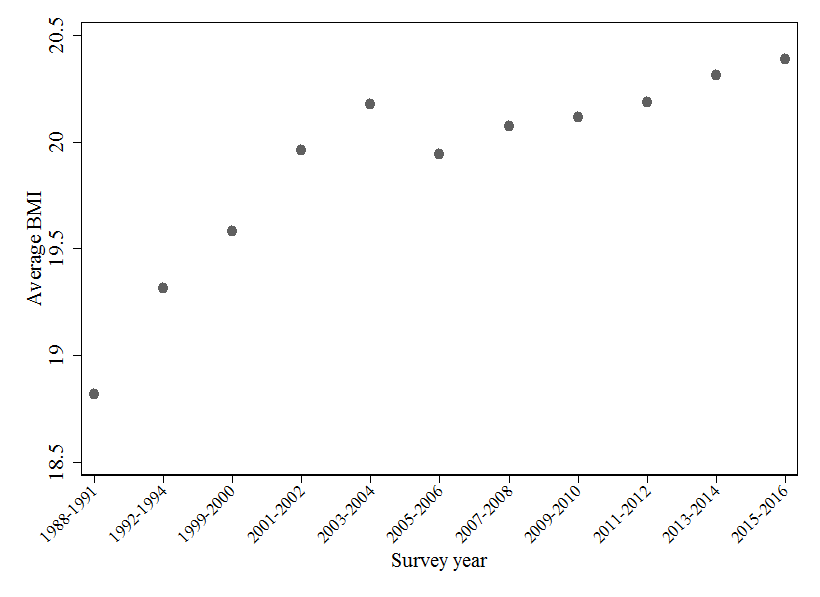
\includegraphics[width=100mm]{Trends_in_obesity_nhanes/output/bmi_2to18_nhanes.png}
  \floatfoot{Notes: Data is from the National Health and Nutrition Examination Survey (NHANES) III and 1999-2016 available at \url{https://www.cdc.gov/nchs/nhanes/index.htm} as of December 2017. The sample is the set of observations between 2 and 18 years of age. The error bars are standard errors that take into account the NHANES stratified sampling design.}
\end{figure}

It is not surprising that fighting childhood obesity has become the focus of many national policies. For example, the Child Nutrition and WIC Reauthorization Act of 2004 aimed to integrate healthy diets and nutritional education into already existing efforts to fight food insecurity, such as the National School Lunch and Breakfast Programs. In particular, the act required that all school districts with a federally funded school meal program designed and implemented wellness policies starting with the 2006/2007 school year. These included physical education and nutrition guidelines that applied to all food available on campus during school days \citep{bauhoff2014effect}.

More recently, the Obama administration has promoted several initiatives to try to respond to the child obesity epidemics. First Lady Michelle Obama's public health campaign ``Let's Move!'' had the stated goal of ``solving the challenge of childhood obesity within a generation so that children born today will reach adulthood at a healthy weight'' \citep{letsmove}. Part of the principles of the Let's Move! campaign were taken up in the Healthy, Hunger-Free Kids Act of 2010. This federal law has given the U.S. Department of Agriculture (USDA) the authority to set new health standards for food sold in school lunches. Some of the consequent changes in at-school meals have been a reduction in portion sizes, and minimum quantities of fruit and vegetables per serving. Moreover, the law has increased program monitoring by requiring school districts to be audited every three years to see if they have met the nutrition standards.

Despite fighting childhood obesity is recognized as one of the challenges of modern society, we still lack a complete understanding of its causes and a clear evaluation of the effectiveness of the attempts made to reduce it so far. This paper tries to fill this gap investigating whether school environment plays a relevant role in determining children obesity status. The main hypothesis is that since kids spend a large fraction of their time at school, exposure to a healthier pool of peers will have strong effects on their behavior, which ultimately could lead to long-lasting changes in weight.

In order to test this theory we will exploit the large geographic variation characterizing the US obesity rate. Figure \ref{fig:adult_vs_childen} shows some first evidence of geographic differences in obesity. Panel A plots the percentage of adult obese population in 2008 by county of residence.
\begin{figure}[htp]
	\centering
	\subfloat[Panel A]{%
  		\includegraphics[clip,width=0.93\columnwidth]{C:/Users/giamb/Google Drive/research projects/obesity/maps/cdc_adult_obesity.png}%
	} \\ \vspace{5mm}
	\subfloat[Panel B]{%
 		\includegraphics[clip,width=0.65\columnwidth]{C:/Users/giamb/Google Drive/research projects/obesity/maps/nhanes_childhood_obesity.png}%
	}
	\caption{Comparison between adult and childhood obesity rates, by county}
	\label{fig:adult_vs_childen}
	\floatfoot{Notes: Panel A shows data on adult obesity from the Centers for Disease Control and Prevention (CDC) available at \url{https://www.cdc.gov/diabetes/atlas/countydata/atlas.html} as of December 2017. Panel B displays data on childhood obesity for all children age 5-17 from Childhood Obesity Index available at \url{http://maps.z-atlas.com/ChildhoodObesityIndex/main.cfm} as of December 2017. Darker-shaded counties have a higher adult or childhood obesity rate in 2008.}
\end{figure}
Panel B similarly plots the county obesity rate for five to seventeen years old children sample in the National Health and Nutrition Examination Survey (NHANES). The absence of a perfect correlation between the two plots shows that there might something else going on other than just family innate preferences.

The identification design discussed in section \ref{identification} tries to disentangle the school environment effect from family choices.

\section{Background}
\label{backgr}
Obesity is usually defined in terms of body mass index (BMI), which is a measure of body mass ($kg$) divided by square body height ($m^2$). For the adult population, normal weight is a BMI between 18.5 and 24.9, overweight is a BMI between 25.0 and 29.9, while obesity is characterized by a BMI over 30. The mapping between BMI and obesity status is slightly different for children 2 to 20 years of age. BMI is usually compared against the percentile for children of the same sex and age computed using NHANES data from 1963 to 1994. A BMI above the relevant $95^{th}$ percentile is considered obese. With these caveats in mind, the next sections will refer to BMI as a synonym for obesity status. Body mass index has the advantage of being a continuous measure as opposed to a 0/1 indicator.

This paper mainly contributes to the literature that tries to identify the economic and social causes of obesity. Looking at the long-term trend in US obesity rate, \cite{cutler2002have} show that the increase in obesity since 1980 was mostly driven by a rise in calories consumed instead of a decline in calories expended. The authors propose a theory based on technical change that shifted the bulk of food preparation from home cooking to mass preparation in restaurant and factories. \cite{eid2008fat} focus instead on the interaction of urban development with obesity. They show that the positive relationship between urban sprawls and obesity documented in other articles is the result of omitted variable bias. More directly related to childhood obesity, \cite{anderson2003economic} claim that for upper income families, mothers working many hours away from home are time constrained and cannot oversee their children's diet and exercise resulting in higher teen obesity rates. 

Another strand of the literature closely related to this project evaluates the effectiveness of school environment and nutrition policies. In a recent working paper, \cite{anderson2017school} suggest that improving the quality of food provided at school improves kids' test scores but does not lead to a decrease in obesity rates. \cite{bauhoff2014effect} uses a synthetic control difference-in-differences method to study the Los Angeles Unified School District's food-and-beverage standards of 2004. He finds that the policy reduced in-school consumption of soda and fried foods but was ineffective at decreasing obesity 8 to 15 months after the intervention. Many articles focus instead on the health outcomes of the National School Lunch (\citealp{gundersen2012impact, campbell2011does}) and Breakfast Programs \citep{bhattacharya2006breakfast}.

A third related literature reports descriptive evidence on adult and childhood obesity. \cite{ogden2016trends} and \cite{iannotti2013trends} are two recent examples of a series of articles that track trends in childhood and adolescents obesity in the US using NHANES or similar survey data. \cite{ng2014global} present a global perspective on the obesity epidemics, while \cite{li2015declining} focus on Massachusetts Public School Districts revealing the existence of wide variation at a local geographic level.

In this paper, I contribute to the literature on childhood obesity in two different ways. First, I adapt the research design recently introduced by \cite{finkelstein2016sources} and exploit children that move between schools to try to disentangle the school environment effect on obesity from innate child or family preferences about nutrition and physical activity. Second, I aim to collect administrative data on children BMI to increase the power of the analysis and be able to exploit the existing variation in obesity rates at a fine geographic level.

\section{Identification strategy and planned estimation}
\label{identification}
The role played by a kid's school environment and social network on her BMI could in principle be studied in a simple cross-sectional framework. For instance, \cite{christakis2007spread} model a person's obesity status as a function of age, sex, and education level. They also allow for network effects on obesity controlling for the obesity status of every other individual to which the person is linked in her network.\footnote{The data used is from the Framingham Offspring Study, which is then connected to the Framingham Heart Study and contains information on 38,611 family and friendship ties for 5209 individuals.} 

To develop a similar framework, let $BMI_{itj}$ define the body mass index of kid $i$ going to school $j$ at time $t$. Let $\tau_t$ be time fixed effects, $\alpha_i$ individual fixed effect, and $\overline{BMI}_{tj}$ the average BMI of other kids in school $j$ excluding child $i$. Let $x_{it}$ denote a vector of control variables that include age, sex, parents' attained education and family income. The naive estimating equation could be written as
\begin{equation}\label{naive}
BMI_{itj} = \alpha_i + \tau_t + \gamma \overline{BMI}_{tj} + x_{it} \beta + \varepsilon_{itj},
\end{equation}
where the parameter of interest is $\gamma$, the coefficient on the average BMI in school $j$.

The cross-sectional estimates could however be biased to the extent that there exists residential sorting. For example, I expect that schools in wealthy neighborhoods will have low average obesity rates. They are also likely correlated with the endogenous availability of healthy food providers and facilities to perform extracurricular physical activities in the area. These can in turn be important variables that help explaining why children going to certain schools have on average lower BMI than their peers in other schools. In presence of such unobserved variables, the estimate of the effect of the average BMI in the school attended by child $i$ will be positively biased.

I try to address this issue exploiting the fact that many students change the school they attend in the early stages of their life. This can happen for two distinct reasons. First, many schools only offer classes for specific grades. For example, most Boston public schools only offer grades K through 5 (elementary schools), grades 6 to 8 (middle schools), or grades 9-12 (high schools). A student enrolled in an elementary school will be forced to move to a different middle school between grades 5 and 6. Following \cite{bradbury2013effect} I denote these transitions as \textit{structural} moves. Second, students might change school for \textit{nonstructural} reasons if, for instance, their families change residential address buying a new house in a different ``school zone''. This might be related to a member of the household finding a better job in a distinct geographic location. I now present a model that can use both structural and nonstructural moves to try to isolate the causal effect of school environment on child obesity status.

Consider a kid $i$ who moves from school $o(i)$ to a different school $d(i)$. Assume first that there is no overall trend in aggregate BMI and that BMI in period $t$ for child $i$ going to school $j$ can be written as a function of individual and school fixed effects, that is 
\begin{equation}
BMI_{itj} = \alpha_i + \gamma_j + \varepsilon_{ijt}.
\end{equation}
I will allow for more complexity in the body mass index equation in the next paragraph. Let $\overline{BMI}_{d(i)}$ and $\overline{BMI}_{o(i)}$ denote the average BMI in the mover's origin and destination school, respectively, and let $\delta_i$ denote the difference between these two. Following \cite{bronnenberg2012evolution} and \cite{finkelstein2016sources} I define the scaled BMI for children $i$ as
\begin{equation}
BMI_{it}^{scaled} = \frac{BMI_{it}-\overline{BMI}_{o(i)}}{\delta_i}.
\end{equation}
Due to scaling, $BMI_{it}^{scaled}$ lies between 0 and 1. It takes a value of 0 if the mover's BMI is equal to the average BMI in her original school. On the other hand, it is equal to 1 if child's BMI and average BMI in the post-move school are equal to each other. Assume now for simplicity that all movers change the school they attend at the same point in time, $t^*$. If the model is correctly specified, the plot of the expectation of $BMI_{it}^{scaled}$ around the move should show a jump at the time of the move and be flat before and after it. Moreover, the mean shift would represent the average value across movers of the share of the difference in BMI between destination and origin that is due to school environment.

I now extent this simplified model to allow for a more precise representation of reality. First, as we already saw in figure \ref{fig:secular_bmi}, the assumption of no overall trend in BMI is not satisfied. Moreover, children BMI is possibly correlated with a set of time varying covariates, such as age, time relative to the move, and family income. To control for these additional variables I assume that the equation governing a child's body mass index can be written as
\begin{equation}
BMI_{itj} = \alpha_i + \gamma_j + \tau_t + x_{it}\beta + \varepsilon_{ijt}.
\end{equation}
Second, it is unlikely that all movers in the sample will be observed for the exact same number of pre- and post-move periods. To avoid introducing spurious pre- or post-trends in the event study figure I thus have to control explicitly for the unbalanced structure of the panel. These two concerns lead to the following event study estimating equation
\begin{equation}\label{event_study}
BMI_{it} = \alpha_i + \theta_{r(i,t)}\hat{\delta}_i + \tau_t + x_{it}\beta + \varepsilon_{it}
\end{equation}
where $\hat{\delta}_i$ denotes the sample analogue of $\delta_i$ computed from the data. The vector of parameters of interest is $\theta_{r(i,t)}$, which indicates the coefficients of the year relative to the move. 

The event study framework based on movers must satisfy three key identification assumptions. First, the underlying reason of the school change must be unrelated with the willingness to change a child's BMI. This assumption would be violated if, for instance, families move to a healthier area -- and consequently kids transition to a healthier school -- with the specific goal of adopting a healthier lifestyle. This concern can be mitigated if we are willing to assume that whenever a family is looking for solutions to fight high BMI we should be able to observe a decrease in weight some periods before the decision of moving to a healthier area (in case this drastic decision is actually taken). This would hence be reflected in a downward sloping pre-trend in the event study plot. Second, the timing of the school change must not correspond with other changes correlated with both the average level of obesity in the destination school and children BMI. For example, this assumption would be violated if a positive income shock leads a family to send its kids to a low obesity rate school and simultaneously to improve the quality of its diet. Third, changes in obesity status influenced by school environment must realize fast after the move and stabilize equally rapidly. Any long lasting post-trend might be an indicator that something other than school environment is driving the change in obesity status. \cite{cutler2002have} illustrate that a very small increase in caloric intake (equivalent to that contained in three Oreo cookies) is sufficient to produce the long-term upward trend in obesity observed in the data. I interpret this as suggestive evidence that changes in diet and physical activity can reflect in abrupt changes in BMI, although this hypothesis can be easily tested in the data. 

To summarize, the ideal event study plot should be flat in the periods before and after the school change. To the extent that there is enough variation between average BMI in the origin and destination schools, structural moves are more suitable to this estimation design than nonstructural ones. In fact, for structural moves, students are exposed to a different school environment \textit{keeping everything else constant}. In other words, using only structural moves would potentially alleviate the first two concerns expressed in the previous paragraph. On the other hand, students changing school due to a structural transition often remain exposed to a similar pool of peers. The spread in average BMI at origin and destination schools might be very low. In this case we will need to complement the analysis with nonstructural moves, which bring back the previous concerns. There are however some ways to test whether the assumptions of the event study framework are satisfied. An idea would be to explore how family income moves around the move. A shift in mean income before and after the school change would be an indicator that the movers design is probably not suitable to study how school environment affects students BMI. 

\section{Data}
To estimate the event study regression described in equation \ref{event_study} we need data on children changing the school environment they are exposed to during the early years of their life. Ideally data should retain information on the school attended by each pupil, her/his grade, measured BMI, and some indicator of family income. Administrative data from states requiring BMI screening would contain most of the variables required for the analysis. They might not collect information on family income. However, this can be partly recovered from average income in the kid's home Zip Code. Figure \ref{fig:admin_data} summarizes states regulations concerning in-school BMI screening as of 2011. 
\begin{figure}[htp]
  \centering
  \caption{US states requiring BMI screening}
  \label{fig:admin_data}
  \includegraphics[width=1\columnwidth]{C:/Users/giamb/Google Drive/research projects/obesity/maps/bmi_screening_states.PNG}
  \floatfoot{Notes: The original table is from \cite{linchey2011peer}.}
\end{figure}
Most of the states mandate BMI screening only in a few grade levels. This limits the power of the event study framework since it would be possible to plot only a few years around the move. Moreover, in many states, each BMI measure is conducted several years after the previous one. Consider for example Massachusetts, where height and weight are measured in grade 1, 4, 7, and 10. Suppose we are looking at students who are registered in a different school between grade 1 and 4. Any mean shift in the event study plot at the time of the move could be hardly interpretable as the causal effect of school environment. Too much time has elapsed between the two measures and there is also no way to determine if the move from the origin to the destination school happened in grade 2 or 3. Moreover, there are also not enough data points to plot credible pre- and post-trends.   

Fortunately, as of 2011, New Jersey and Pennsylvania required BMI screening in each grade 1 through 12. If we consider both structural and nonstructural moves of students changing school between grade 5 and 6 we will have enough observations to construct reasonable pre-and post-trends. 

A caveat to keep in mind using administrative data from different states is that it might be hard to identify kids moving across states. However, moves within each state might be enough to uncover the causal effect of school environment on students obesity status. For this to be true we need enough variation in average school BMI within a given state. Figure \ref{fig:ny_obesity} shows that there are large difference in obesity rate at the school district level in the state of New York. This is likely to be true for every other large US state.\footnote{We already saw in section \ref{backgr} that \cite{li2015declining} report similarly wide variation in childhood obesity rates in Massachusetts Public School Districts.}  
\begin{figure}[htp]
  \centering
  \caption{Differences in childhood obesity rate in New York school districts}
  \label{fig:ny_obesity}
  \includegraphics[width=110mm]{C:/Users/giamb/Google Drive/research projects/obesity/maps/childhood_obesity_ny.PNG}
  \floatfoot{Notes: Data is from the New York State Department of Health available at \url{https://health.data.ny.gov/Health/Student-Weight-Percent-Obese-by-School-District-Ma/i9hu-ki7z\#revert} as of December 2017. Darker shaded areas indicate school districts with a higher percentage of obese students.}
\end{figure}

Although administrative data are ideal in terms of number of observations and reliability, they come with the shortcoming of being hard to access. Fortunately, the Early Childhood Longitudinal Study (ECLS-K) and the National Longitudinal Survey of Youth 1979 (NLSY79) can be used as alternative source of data in the same estimation design.

The ECLS-K follows students from the kindergarten class of 1998-1999 through 8th grade. The study is nationally representative and it includes about 22,700 children sampled from 1,300 schools in the 1998-1999 school year. Data is collected two times when the children are in kindergarten (1998-1999) and in first grade (1999-2000), and once during the third grade (2002), fifth grade (2004), and eighth grade (2007) school years.  The data contains useful information on children's early behavior including information on food consumption in and out of school, as well as different measures of physical activity. For example, the questionnaire contains questions on consumption of fruits, vegetables, soda, milk and other foods for all meals consumed during the seven days before the interview. It also asks questions related to the type of food available at school and whether the family participates in the national school lunch program or breakfast program. We also encounter questions on the frequency of physical activity each week and participation in extracurricular activities. Most importantly, the children's weight and height at the time of the interview are actually measured by the interviewer. This prevents the issue of over reporting height and under reporting weight common to self-reported survey data. 

It is interesting to notice that by looking at changes in school identifier I computed that about 2,540 students moved between the spring of the first grade and the spring of the third grade. This is roughly in line with the 10.6\% nonstructural school changes estimated by \citep{bradbury2013effect} for non high school Boston Public School students. Restricted use data contain information on census tract and Zip Code for children's homes and schools, which allow to control for more detailed geographic characteristics.

Similar to the ECLS-K, the Early Childhood Longitudinal Study 2011 (ECLS-K:2011) follows a nationally representative sample of the US kindergarten class of 2010-11 as they progress through their fifth grade. The data is collected in the fall and the spring of kindergarten (2010-2011), the fall and spring of 1st grade (2011-2012), the fall and spring of 2nd grade (2012-2013), the spring of 3rd grade (2014), the spring of 4th grade (2015), and the spring of 5th grade (2016). The sample size is of approximately 20,230 children from 1,320 schools.

The NLSY79 is a second useful alternative to administrative data. It contains information on a sample of 12,686 individuals who were age 14 to 22 in 1979. Interviews were conducted annually from 1979 through 1994 and biennially until 2012. Interestingly, this survey can be linked to the NLSY-Children and Young Adults to study approximately 11,500 children who were born to female NLSY-79 respondents. 

\newpage
\bibliography{Report}


\end{document}